\chapter{Riflessione e rifrazione delle onde}%Riflessione e rifrazione delle onde
\section{Teoremi fondamentali}%Teoremi fondamentali
L'incidenza di un'onda sulla superficie di separazione tra due mezzi dà origine a un'onda riflessa che si propaga all'indietro nello stesso mezzo in cui si propaga l'onda incidente e ad un'onda rifratta (trasmessa) che si propaga nel secondo mezzo.

\subsection{Teorema di Kirchhoff}
\begin{teo}[di Kirchhoff]
\b{La perturbazione $\xi_P\(t\)$ prodotta da un insieme di sorgenti in un punto $P$ si può calcolare}, pur ignorando la distribuzione spaziale delle sorgenti, \b{quando}, data una superficie chiusa $\Sigma$ arbitraria che racchiude le sorgenti, \b{si conoscano i valori di $\xi$ e della sua derivata normale $\frac{\partial\xi}{\partial n}$ in tutti i punti di $\Sigma$}.
\end{teo}

Si definisce \b{perturbazione}:
\begin{equation}\begin{split}
\xi\(q,t\)=\frac{q_0\xi_0}{q}\cos{\(kq-\omega t\)}=\frac{q_0\xi_0}{q}\cos{\[\omega\(\frac{q}{v}-t\)\]}
\end{split}\end{equation}
essendo $q$ la distanza da un punto qualsiasi dalla sorgente.

Il \b{teorema di Kirchhoff} dà alla perturbazione in un punto $P$ distante $r$ dalla sorgente e $s$ da un altro punto l'espressione:
\begin{equation}\begin{split}
\xi_P\(r,t\)=\\
\frac{\xi_0}{2\lambda}\oint{\frac{1}{qs}\(\cos{\theta_0}+\cos{\theta}\)\cos{\[k\(q+s\)-\omega t-\frac{\pi}{2}\]}d\Sigma}=\\
\oint{\frac{A}{s}f\(\theta\)\cos{\[k\(q+s\)-\omega t-\frac{\pi}{2}\]}d\Sigma}
\end{split}\end{equation}
essendo $\lambda$ la lunghezza d'onda e nell'ultimo passaggio si suppone che $\Sigma$ coincida con una superficie d'onda sferica di raggio $q$ emessa dalla sorgente posta al centro di $\Sigma$ e ponendo $A=\frac{\xi_0}{\lambda q}$ come \b{ampiezza} e $f\(\theta\)=\frac{1+\cos{\theta}}{2}$ come \b{fattore di obliquità} o \b{di inclinazione}.

Si definiscono \b{onda sferica infinitesima} la quantità:
\begin{equation}\begin{split}
d\xi_P=\frac{A}{s}f\(\theta\)d\Sigma\cos{\[k\(q+s\)-\omega t-\frac{\pi}{2}\]}=dA^*\cos{\[k\(q+s\)-\omega t-\frac{\pi}{2}\]}
\end{split}\end{equation}
e \b{ampiezza infinitesima} la quantità:
\begin{equation}\begin{split}
dA^*=\frac{A}{s}f\(\theta\)d\Sigma=\xi_0\frac{f\(\theta\)d\Sigma}{\lambda qs}.
\end{split}\end{equation}

\subsection{Principio di Huygens-Fresnel}
\begin{teo}[Principio di Huygens-Fresnel]
\b{Ogni elemento $d\Sigma$ di una superficie d'onda $\Sigma$ si può considerare} formalmente \b{come una sorgente di onde secondarie sferiche la cui ampiezza}, proporzionale all'ampiezza dell'onda primaria e all'area $d\Sigma$, \b{varia con l'angolo secondo la funzione $f\(\theta\)$}. \b{La perturbazione prodotta in un punto $P$ si può sempre ottenere come sovrapposizione di tutte le onde sferiche elementari che raggiungono $P$}.
\end{teo}

Esso è uno strumento di calcolo molto utile: si determina un nuovo fronte d'onda ad un certo istante a partire da un fronte d'onda precedente.

\subsubsection{Onda attraverso uno spazio libero}
Noto all'istante $t$ il fronte d'onda $\Sigma$, piano o sferico, per costruire il fronte d'onda in un istante successivo si considerano i punti di $\Sigma$ come sorgenti di onde sferiche secondarie, emesse tutte nello stesso istante. Per ogni punto si traccia una semicirconferenza di raggio $v\(t'-t\)=v\Delta t$ e il nuovo fronte d'onda, luogo dei punti di fase uguale, risulta essere l'inviluppo di tutte queste onde.

\subsubsection{Onda incontra uno schermo impenetrabile con un'apertura}
Si può calcolare il fronte d'onda al di là dell'apertura eliminando le sorgenti che stanno su quella parte del fronte che non coincide con l'apertura. Se \b{l'apertura ha una larghezza grande rispetto alla lunghezza d'onda}, l'onda che emerge dall'apertura conserva la forma del fronte d'onda incidente: \b{propagazione rettilinea}. Se \b{l'apertura ha una larghezza confrontabile con la lunghezza d'onda}, l'onda uscente tende a propagarsi in tutte le direzioni: \b{diffrazione}.

\subsubsection{Onda incontra uno schermo impenetrabile che coincide con un fronte d'onda con $n$ aperture}
Se tutte le aperture hanno la stessa area $d\Sigma$, si ottiene un sistema di $n$ sorgenti di onde sferiche, ciascuna di ampiezza $dA^*$. Preso un punto oltre lo schermo che dista $s_i$ da $S_i$ e $s_j$ da $S_j$, la \b{differenza di fase} in $P$ delle due onde emesse risulta \b{costante nel tempo}:
\begin{equation}\begin{split}
\phi_{i,j}=\[k\(q+s_i\)-\omega t-\frac{\pi}{2}\]-\[k\(q+s_j\)-\omega t-\frac{\pi}{2}\]=k\(s_i-s_j\).
\end{split}\end{equation}

\section{Leggi della riflessione e della rifrazione}%Leggi della riflessione e della rifrazione
Se l'onda è armonica, caratterizzata da frequenza, pulsazione, lunghezza d'onda e numero d'onda, \b{nell'attraversamento della superficie pulsazione e frequenza non variano}, in quanto determinate dalla sorgente che ha prodotto l'onda, \b{e di conseguenza variano la lunghezza d'onda e il numero d'onda}:
\begin{equation}\begin{split}
\omega=2\pi\nu, \qquad v=\lambda\nu, \qquad k=\frac{\omega}{v}=\frac{2\pi}{\lambda}, \qquad \frac{\lambda_1}{\lambda_2}=\frac{v_1}{v_2}, \qquad \frac{k_1}{k_2}=\frac{v_2}{v_1}.
\end{split}\end{equation}

Per \b{un'onda \elettrom che passi dal vuoto ad un mezzo trasparente} valgono le relazioni:
\begin{equation}\begin{split}
\lambda=\frac{\lambda_0}{n}, \qquad k=\frac{2\pi}{\lambda_0}n=k_0n
\end{split}\end{equation}
cioè \b{la lunghezza d'onda in un mezzo è sempre minore della lunghezza d'onda nel vuoto}.

\subsection{Onda piana}
Viene descritta da:
\begin{equation}\begin{split}
\xi_i=\xi_0\cos{\(\k_i\cdot\r-\omega t\)}.
\end{split}\end{equation}
che si muove nella direzione $\k_i$.

Dall'onda incidente ha origine un'\b{onda riflessa}:
\begin{equation}\begin{split}
\xi_r=\xi_{0_{r}}\cos{\(\k_r\cdot\r-\omega t\)}
\end{split}\end{equation}
e un'\b{onda rifratta}:
\begin{equation}\begin{split}
\xi_t=\xi_{0_{t}}\cos{\(\k_t\cdot\r-\omega t\)}
\end{split}\end{equation}
che si muovono rispettivamente nelle direzioni $\k_r$ e $\k_t$.

\b{Sulla superficie di separazione, le fasi delle tre onde devono risultare in ogni istante uguali}:
\begin{equation}\begin{split}
\k_i\cdot\r=\k_r\cdot\r=\k_t\cdot\r.
\end{split}\end{equation}

\subsection{Superficie di separazione coincidente con piano $xy$}
Il vettore $\k_i$ giace nel piano $yz$. Si ottiene quindi:
\begin{equation}\begin{split}
\r=x\u_x+y\u_y, \qquad \k_i=k_{i,y}\u_y+k_{i,z}\u_z\\
\Longrightarrow k_{i,y}y=k_{r,x}x+k_{r,y}y=k_{t,x}x+k_{t,y}y\\
\Longrightarrow k_{r,x}=k_{t,x}=0, \qquad k_{i,y}=k_{r,y}=k_{t,y}.
\end{split}\end{equation}

Si definisce il \b{piano di incidenza} il piano ortogonale alla superficie di separazione individuato da $\k_i$ e da $\u_z$.

\begin{teo}[Prima legge della riflessione e della rifrazione]
Le direzioni di propagazione dell'onda incidente, dell'onda riflessa e dell'onda rifratta giacciono nel piano di incidenza, individuato dalla direzione di incidenza e dalla normale alla superficie di separazione nel punto di incidenza.
\end{teo}

Considerando $k_{i,y}=k_i\sin{\theta_i}=\frac{\omega}{v_1}\sin{\theta_i}$, $k_{r,y}=\frac{\omega}{v_1}\sin{\theta_r}$ e $k_{t,y}=\frac{\omega}{v_2}\sin{\theta_2}$ e inserendo in $k_{i,y}=k_{r,y}=k_{t,y}$ si ottiene $\sin{\theta_i}=\sin{\theta_r}$ e $\frac{1}{v_1}\sin{\theta_i}=\frac{1}{v_2}\sin{\theta_t}$, che permette di definire la \b{relazione di riflessione} data dal teorema:
\begin{teo}[Seconda legge della riflessione e della rifrazione]
L'angolo di riflessione è uguale all'angolo di incidenza.
\begin{equation}\begin{split}
\theta_i=\theta_r
\end{split}\end{equation}
\end{teo}

Si ha anche la \b{relazione di rifrazione} data dal teorema:
\begin{teo}[Terza legge della riflessione e della rifrazione]
Il rapporto tra il seno dell'angolo di incidenza e il seno dell'angolo di rifrazione è costante ed uguale al rapporto tra le velocità di propagazione.
\begin{equation}\begin{split}
\frac{\sin{\theta_i}}{\sin{\theta_t}}=\frac{v_1}{v_2}.
\end{split}\end{equation}
\end{teo}

\subsection{Riflessione e rifrazione della luce}
Per un'onda luminosa piana che attraversa la superficie di separazione tra due mezzi trasparenti è la partenza della \b{legge di Snell}:
\begin{equation}\begin{split}
\frac{\sin{\theta_i}}{\sin{\theta_t}}=\frac{v_1}{v_2}=\frac{c}{n_1}\frac{n_2}{c}=\frac{n_2}{n_1}=n_{2,1}\\
\Longrightarrow n_1\sin{\theta_i}=n_2\sin{\theta_t}
\end{split}\end{equation}
che, dopo aver definito \b{indice di rifrazione relativo del secondo mezzo rispetto al primo} il valore $n_{2,1}$, enuncia che:
\begin{teo}[Legge di Snell]
Il \b{rapporto tra il seno dell'angolo di incidenza e il seno dell'angolo di rifrazione è costante} ed \b{uguale all'indice di rifrazione relativo tra i due mezzi}.
\end{teo}

\subsection{Riflessione totale}
\subsubsection{Onda luminosa piana si propaga da un mezzo con indice di rifrazione $n_1$ ad un mezzo con indice di rifrazione $n_2>n_1$}
Si ha:
\begin{equation}\begin{split}
\sin{\theta_2}=\frac{n_1}{n_2}\sin{\theta_1}\\
\Longrightarrow \theta_2<\theta_1.
\end{split}\end{equation}
Nell'attraversamento la direzione di propagazione dell'onda trasmessa si avvicina alla normale.

\subsubsection{Onda luminosa piana si propaga da un mezzo con indice di rifrazione $n_1$ ad un mezzo con indice di rifrazione $n_2<n_1$}
Si ha:
\begin{equation}\begin{split}
\sin{\theta_2}=\frac{n_1}{n_2}\sin{\theta_1}\\
\Longrightarrow \theta_2>\theta_1.
\end{split}\end{equation}
Nell'attraversamento la direzione di propagazione dell'onda trasmessa si allontana dalla normale.

In questo caso si ha il \b{caso limite}: al crescere dell'angolo di incidenza $\theta_1$, l'angolo di trasmissione $\theta_2$, che cresce più rapidamente, raggiunge ad un certo punto il valore $\frac{\pi}{2}$, in corrispondenza del valore $\theta_0$ chiamato \b{angolo limite}:
\begin{equation}\begin{split}
\sin{\theta_0}=\frac{n_2}{n_1}.
\end{split}\end{equation}
Si ha quindi che \b{per valori di $\theta_1$ maggiori di $\theta_0$ non esistono valori reali di $\theta_2$ e perciò l'onda rifratta non si forma più e quindi l'onda incidente è totalmente riflessa all'interno del primo mezzo}.

Un utilizzo interessante si ha nel trasporto di un fascio luminoso tramite una guida di luce costituita da un cilindro pieno di vetro o di materiale plastico trasparente immerso in un mezzo con indice di rifrazione inferiore o attraverso fibre ottiche. La luce che penetra nel cilindro attraverso una base incide sulle pareti laterali formando un angolo superiore all'angolo limite e viene riflessa totalmente molte volte, senza apprezzabili perdite, fino ad uscire dall'altra base.

\subsection{Dispersione della luce in un mezzo trasparente}
Il rapporto $\frac{\sin{\theta_i}}{\sin{\theta_t}}$ è costante se la luce incidente ha una sola lunghezza d'onda, cioè se è monocromatica. Qualora siano contenute più lunghezze d'onda, ad un dato angolo di incidenza corrispondono più angoli di rifrazione.

Esiste una dipendenza dell'indice di rifrazione dalla lunghezza d'onda definito dalla \b{legge di Cauchy}:
\begin{equation}\begin{split}
n\(\lambda\)=A+\frac{B}{\lambda^2}.
\end{split}\end{equation}
L'\b{indice diminuisce al crescere della lunghezza d'onda}, per cui, a parità di $\theta_i$, $\theta_t$ è più piccolo per il violetto che per il rosso: il raggio rifratto violetto è più vicino alla normale e quindi è più deviato di quanto lo sia il raggio rosso.
\begin{center}
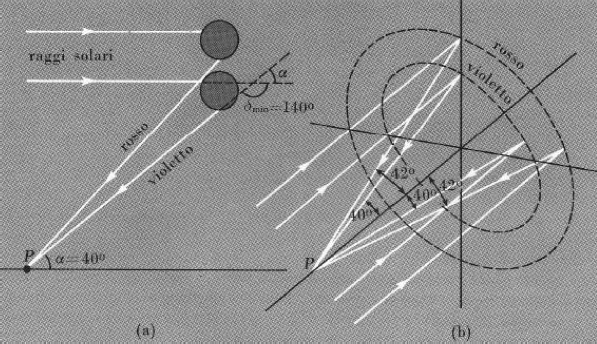
\includegraphics[width=\textwidth]{immagini/dispersione1.png}
\end{center}
\begin{center}
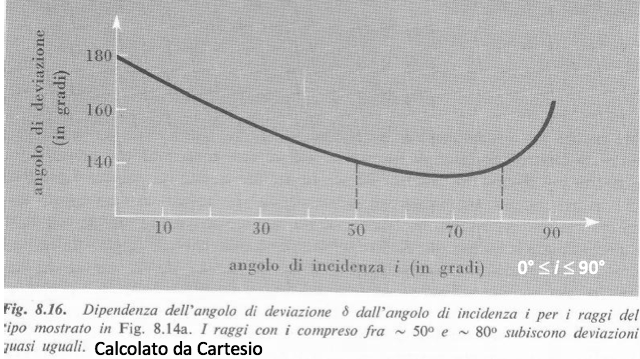
\includegraphics[width=\textwidth]{immagini/dispersione2.png}
\end{center}

\subsubsection{Miraggio}
Se la temperatura dell'aria cresce andando verso terra, la densità e l'indice di rifrazione aumentano andando verso l'alto. Si vedono perciò due raggi, e immaginando che uno sia riflesso, si pensa ci sia l'acqua.
\begin{center}
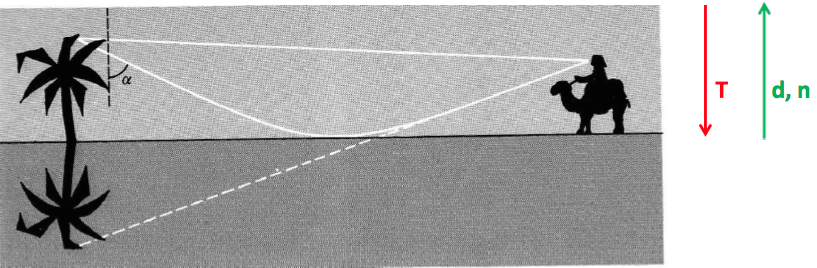
\includegraphics[width=\textwidth]{immagini/miraggio.png}
\end{center}

\subsubsection{Fata Morgana}
\'E l'opposto del miraggio. In questo caso però si vede l'oggetto ``volare''.
\begin{center}
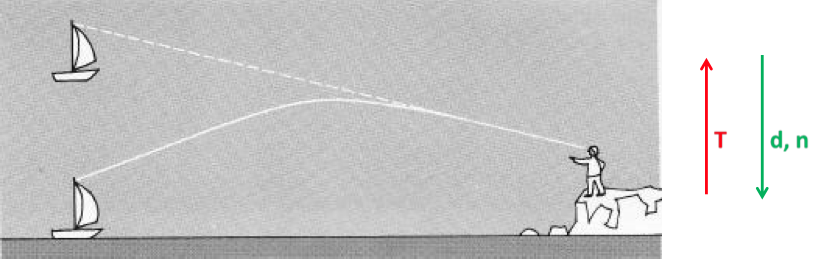
\includegraphics[width=\textwidth]{immagini/morgana.png}
\end{center}

\subsubsection{Arcobaleni}
Se si vedono due arcobaleni insieme, uno ha i colori giusti, l'altro invertiti. Si vedono spesso di sera gli arcobaleni perché alle 17.00 c'è più probabilità che piova.
\begin{center}
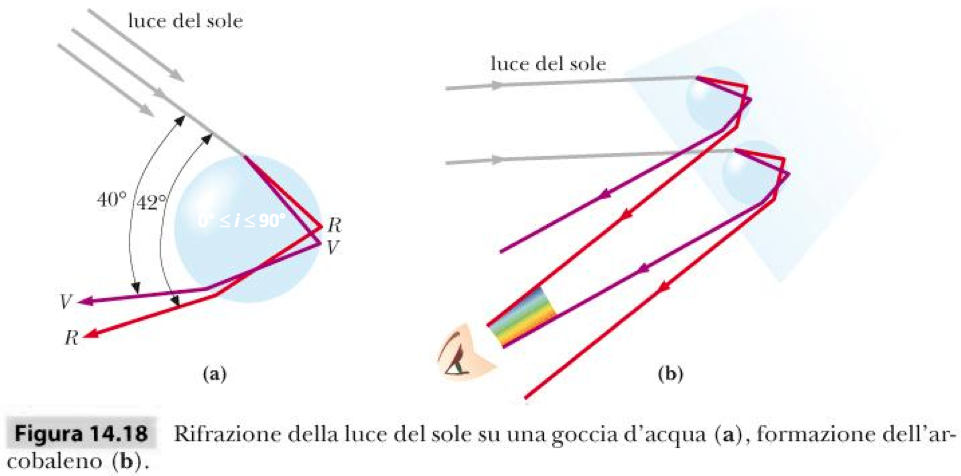
\includegraphics[width=\textwidth]{immagini/arcobaleno1.png}
\end{center}
Se il sole è più alto di \ang{41;;} da terra non si vede più l'arcobaleno. Se l'osservatore si alza da terra aumenta l'arco visibile.
\begin{center}
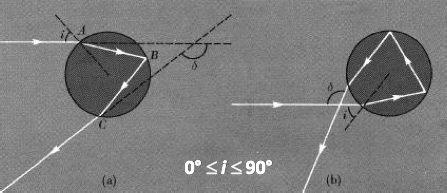
\includegraphics[width=\textwidth]{immagini/arcobaleno2.png}
\end{center}

\subsubsection{Ionosfera}
Si chiama così quella parte dell'atmosfera situata all'incirca tra \SI{100}{\kilo\metre} e \SI{400}{\kilo\metre} dalla superficie terrestre, in cui l'aria è parzialmente ionizzata per l'azione della radiazione ultravioletta proveniente dal sole. Il gas è complessivamente neutro, anche se una qualsiasi perturbazione può causare una separazione locale delle cariche: non appena questa separazione avviene, agisce una forza elettrica di richiamo sulle cariche. Con buona approssimazione si può considerare solo il moto degli elettroni e immaginare la situazione seguente: da una zona neutra si è avuto uno spostamento di elettroni che dà origine a uno strato carico negativamente e lascia dall'altra parte uno strato carico positivamente.

\begin{center}
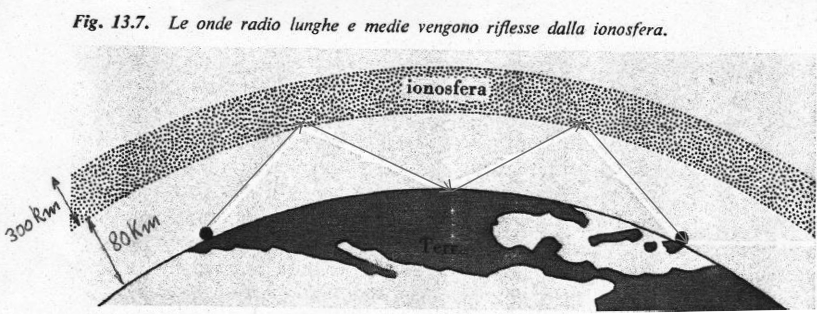
\includegraphics[width=\textwidth]{immagini/ionosfera.png}
\end{center}

Se $N$ è il numero di cariche libere per unità di volume e $x$ lo spessore dello strato carico, questo equivale ad una distribuzione superficiale di carica (con densità $Nex$), per cui il campo elettrico nello spazio intermedio è $E=\frac{Nex}{\e_0}$. La forza sugli elettroni è $-eE$ e ricavata l'equazione del moto si ha che, una volta causata la perturbazione, ha luogo un moto armonico con pulsazione $\omega=\sqrt{\frac{Ne^2}{\e_0m_e}}=\omega_p\simeq \SI{e8}{rad/s}$ e frequenza $\nu_p=\frac{\omega_p}{2\pi}=\simeq\SI{18.7}{m}$.

\section{Intensità delle onde elettromagnetiche riflesse e rifratte}%Intensità delle onde elettromagnetiche riflesse e rifratte
Si hanno le relazioni:
\begin{equation}\begin{split}
\theta_i=\theta_r, \qquad \frac{\sin{\theta_i}}{\sin{\theta_t}}=\frac{n_2\(\omega\)}{n_1\(\omega\)}=\sqrt{\frac{\ke_2\(\omega\)}{\ke_1\(\omega\)}}.
\end{split}\end{equation}

Le relazioni tra le ampiezze si ricavano dalle condizioni di continuità delle equazioni di Maxwell. Dati due dielettrici omogenei e isotropi di costanti dielettriche $\e_1=\e_0\ke_1$ e $\e_2=\e_0\ke_2$ e permeabilità magnetiche $\mu_1$ e $\mu_2$, è possibile stabilire relazioni tra le componenti del campo elettrico $\E$, dell'induzione dielettrica $\D$, del campo magnetico $\B$ e del campo $\H$ in un mezzo e nell'altro, in punti molto vicini alla superficie di separazione $\Sigma$ tra i mezzi:
\begin{equation}\begin{split}
\begin{cases}
\frac{D_{1,p}}{\e_0\ke_1}=E_{1,p}=E_{2,p}=\frac{D_{1,p}}{\e_0\ke_2}\\
H_{1,p}=\frac{B_{1,p}}{\mu_1}=\frac{B_{2,p}}{\mu_2}=H_{2,p}
\end{cases}
\qquad
\begin{cases}
D_{1,n}=\e_0\ke_1E_{1,n}=\e_0\ke_2E_{2,n}=D_{2,n}\\
B_{1,n}=\mu_1H_{1,n}=\mu_2H_{2,n}=B_{2,n}
\end{cases}
\end{split}\end{equation}
cioè \b{sono continue le componenti parallele di \dE e di $\H$ e le componenti normali di \dD e di $\B$, discontinue le altre}.

Sulla superficie $\Sigma$ incide un'onda \elettrom piana $\E_i=\E_{0,i}\sin{\(\k_i\cdot\r-\omega t\)}$ che dà origine ad un'onda riflessa $\E_r=\E_{0,r}\sin{\(\k_r\cdot\r-\omega t\)}$ e un'onda rifratta $\E_t=\E_{0,t}\sin{\(\k_t\cdot\r-\omega t\)}$. Su $\Sigma$, l'onda riflessa si somma all'onda incidente dando il campo elettrico risultante nel primo mezzo:
\begin{equation}\begin{split}
\E_1=\E_i+\E_r;
\end{split}\end{equation}
nel secondo mezzo il campo elettrico vale $\E_2=\E_t$. Analoghe relazioni valgono per il campo magnetico nel primo mezzo:
\begin{equation}\begin{split}
\B_1=\B_i+\B_r
\end{split}\end{equation}
e nel secondo $\B_2=\B_t$.

\subsection{Incidenza normale alla superficie di separazione}
Consideriamo il caso più semplice di un'onda \elettrom piana monocromatica che si propaga in un mezzo con indice di rifrazione $\widetilde n_0$ e che incide sulla superficie di un mezzo semi-infinito con indice di rifrazione $\widetilde n$, non magnetico ($\mu=\mu_0$).

Condizioni al contorno per le componenti tangenziali di \dE e \dH (con $\E=\mu_0\H\times\v$ e quindi $\H=\frac{\E}{\mu_0\v}$) dell'onda incidente ($i$), riflessa ($r$) e rifratta ($t$) sono:
\begin{equation}\begin{split}
\begin{cases}
\widetilde E_t=\widetilde E_i+\widetilde E_r\\
\widetilde n\widetilde E_t=\widetilde n_i\widetilde E_i+\widetilde n_i\widetilde E_r
\end{cases}
\end{split}\end{equation}
e risolvendo per $\widetilde E_r$ e $\widetilde E_t$ si hanno i \b{coefficienti complessi di Fresnel in riflessione e rifrazione}:
\begin{equation}\begin{split}
\begin{cases}
\widetilde r=\frac{\widetilde E_r}{\widetilde E_i}=\frac{\widetilde n_i-\widetilde n}{\widetilde n_i+\widetilde n}\\
\widetilde t=\frac{\widetilde E_t}{\widetilde E_i}=\frac{2\widetilde n_i}{\widetilde n_i+\widetilde n}.
\end{cases}
\end{split}\end{equation}
Con $\widetilde n$ si indica il coefficiente del secondo mezzo.

$\widetilde r$ e $\widetilde t$ sono generalmente grandezze complesse e quindi le onde riflesse e trasmesse cambiano in ampiezza e fase rispetto all'onda incidente. $\widetilde r$ cambia solo in segno invertendo la direzione di propagazione, $\widetilde t$ cambia in valore assoluto e
\begin{equation}\begin{split}
\widetilde t=1+\widetilde r.
\end{split}\end{equation}

Nei mezzi trasparenti ($n_i$ e $n$ reali), con $n_i<n$, in riflessione si ha un cambio di fase pari a $\pi$.

All'interfaccia tra i due mezzi, le intensità $I_r$ dell'onda riflessa e $I_t$ dell'onda rifratta (trasmessa), relative all'intensità $I_i$ dell'onda incidente definiscono la \b{riflettività}:
\begin{equation}\begin{split}
R=\frac{I_r}{I_i}=|\widetilde r|^2=\left|\frac{\widetilde n_i-\widetilde n}{\widetilde n_i+\widetilde n}\right|^2=\frac{\(n-n_i\)^2+\(\ke-\e_0\)^2}{\(n+n_i\)^2+\(\ke+\e_0\)^2}
\end{split}\end{equation}
e la \b{trasmittività}:
\begin{equation}\begin{split}
T=\frac{I_t}{I_i}=\Re{\(\frac{\widetilde n}{\widetilde n_i}\)}\left|\widetilde t\right|=\Re{\(\frac{\widetilde n}{\widetilde n_i}\)}\left|\frac{2\widetilde n_i}{\widetilde n_i+\widetilde n}\right|.
\end{split}\end{equation}

$R$ e $T$ sono entrambi minori di 1, e la loro somma dà $R+T=1$.

Vengono definite anche la \b{riflettanza}:
\begin{equation}\begin{split}
\mathcal{R}=R+\frac{\(1-R^2\)Re^{-2\alpha d}}{1-R^2e^{-2\alpha d}}
\end{split}\end{equation}
e la \b{trasmittanza}:
\begin{equation}\begin{split}
\mathcal{T}=\frac{\(1-R^2\)e^{-\alpha d}}{1-R^2e^{-2\alpha d}}
\end{split}\end{equation}
e infine l'\b{assorbanza} $\mathcal{A}=1-\mathcal{R}-\mathcal{T}$. Solo quando $\alpha d\gg1$ si ha $\mathcal{R}$ ha solo il primo termine e coincide con $R$ e $\mathcal{T}\sim0$. \b{\'E stata fatta una somma incoerente delle onde riflesse e trasmesse}.

\subsubsection{Somma coerente dei campi}
La risposta ottica di un film delimitato da due superfici rigorosamente piane parallele è ottenuta sommando coerentemente i campi elettrici riflessi e trasmessi, cioè i contributi dei coefficienti complessi di Fresnel $\widetilde r$ e $\widetilde t$:
\begin{equation}\begin{split}
\widetilde r=\\
\widetilde r_{0,1}+\\
\widetilde t_{0,1}e^{i\frac{2\pi}{\lambda}\widetilde n\cdot x}\widetilde r_{1,2}e^{i\frac{2\pi}{\lambda}\widetilde n\cdot x}\widetilde t_{1,0}+\\
\widetilde t_{0,1}e^{i\frac{2\pi}{\lambda}\widetilde n\cdot x}\widetilde r_{1,2}e^{i\frac{2\pi}{\lambda}\widetilde n\cdot x}\widetilde r_{1,0}e^{i\frac{2\pi}{\lambda}\widetilde n\cdot x}\widetilde r_{1,2}e^{i\frac{2\pi}{\lambda}\widetilde n\cdot x}\widetilde t_{1,0}+\dots
\end{split}\end{equation}
\begin{equation}\begin{split}
\widetilde t=\\
\widetilde t_{0,1}e^{i\frac{2\pi}{\lambda}\widetilde n\cdot x}\widetilde t_{1,2}+\\
\widetilde t_{0,1}e^{i\frac{2\pi}{\lambda}\widetilde n\cdot x}\widetilde r_{1,2}e^{i\frac{2\pi}{\lambda}\widetilde n\cdot x}\widetilde r_{1,0}e^{i\frac{2\pi}{\lambda}\widetilde n\cdot x}\widetilde t_{1,2}+\\
\widetilde t_{0,1}e^{i\frac{2\pi}{\lambda}\widetilde n\cdot x}\widetilde r_{1,2}e^{i\frac{2\pi}{\lambda}\widetilde n\cdot x}\widetilde r_{1,0}e^{i\frac{2\pi}{\lambda}\widetilde n\cdot x}\widetilde r_{1,2}e^{i\frac{2\pi}{\lambda}\widetilde n\cdot x}\widetilde r_{1,0}e^{i\frac{2\pi}{\lambda}\widetilde n\cdot x}\widetilde t_{1,2}+\dots\\
\end{split}\end{equation}
e ciascun termine è descritto dall'ampiezza $|a|=\sqrt{|\widetilde a\cdot\widetilde a^*|}$ e dalla fase $\phi=\arctan{\(\frac{\Im{\(\widetilde a\)}}{\Re{\(\widetilde a\)}}\)}$.

La riflettanza (e la trasmittanza) sono date dal modulo quadro della somma di tutti i termini, tenendo conto della loro fase, ottenendo così gli effetti di interferenza:
\begin{equation}\begin{split}
I=\left|\sum_{n=0}^\infty{\widetilde a_n}\right|
\end{split}\end{equation}
essendo l'informazione sulla fase contenuta nei termini misti. Quando le inomogeneità della superficie o del campione, così come le rugosità o le variazioni dello spessore, distruggono la coerenza di fase, l'informazione sulla fase è persa (almeno parzialmente).

%\subsubsection{Modello di Lorentz}
%
%\subsubsection{Modello di Drude}
%

\subsection{Intensità riflessa e rifratta - caso generale}
Per trovare i coefficienti di Fresnel nel caso generale di un'onda piana monocromatica che si propaga in un mezzo con indice di rifrazione $\widetilde n_i$, incidente con un angolo $\phi_0$ su un mezzo semi-infinito con indice di rifrazione $\widetilde n$, conviene, senza perdita di generalità, scomporre sia \dE sia \dH in componenti perpendicolari (pedice $s$=secante) e parallele ($p$) al piano di incidenza.
\begin{center}
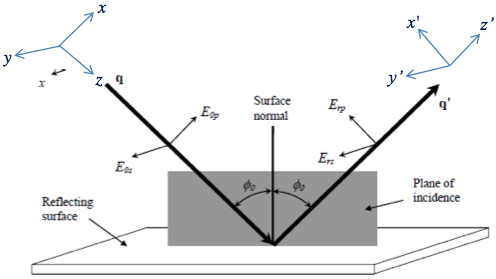
\includegraphics[width=4.5in]{immagini/rifrifra-obl.png}
\end{center}
Nel sistema di coordinate locali $\(x,y,z\)$ il campo incidente $\widetilde \E_i\(\r,t\)$ lungo la direzione $z$ può essere
rappresentato come
\begin{equation}\begin{split}
\widetilde \E_i\(\r,t\)=\(\widetilde E_{i,p}\bb{i}+\widetilde E_{i,s}\bb{j}\)e^{i\(\widetilde \q\cdot\r-\omega t\)}.
\end{split}\end{equation}

Il campo elettrico dell'onda riflessa e, analogamente, quello dell'onda rifratta, può essere espresso in un altro sistema di coordinate locali da:
\begin{equation}\begin{split}
\widetilde \E_r\(\r',t\)=\(\widetilde E_{i,p}\widetilde r_p\bb{i}'+\widetilde E_{i,s}\widetilde r_s\bb{j}'\)e^{i\(\widetilde \q'\cdot\r'-\omega t\)}
\end{split}\end{equation}
\begin{equation}\begin{split}
\widetilde \E_t\(\r',t\)=\(\widetilde E_{i,p}\widetilde t_p\bb{i}'+\widetilde E_{i,s}\widetilde t_s\bb{j}'\)e^{i\(\widetilde \q'\cdot\r'-\omega t\)}.
\end{split}\end{equation}

Come per incidenza normale, imponendo le condizioni di continuità all'interfaccia per \dE e \dH si ottengono i \b{coefficienti complessi di Fresnel in riflessione}:
\begin{equation}\begin{split}
\begin{cases}
\widetilde r_p=\frac{\widetilde E_{r,p}}{\widetilde E_{i,p}}=\frac{\widetilde n_i\cos{\widetilde \phi}-\widetilde n\cos{\widetilde \phi_0}}{\widetilde n_i\cos{\widetilde \phi}+\widetilde n\cos{\widetilde \phi_0}}\\
\widetilde r_s=\frac{\widetilde E_{r,s}}{\widetilde E_{i,s}}=\frac{\widetilde n_i\cos{\widetilde \phi_0}-\widetilde n\cos{\widetilde \phi}}{\widetilde n_i\cos{\widetilde \phi_0}+\widetilde n\cos{\widetilde \phi}}
\end{cases}
\end{split}\end{equation}
\b{e in trasmissione}:
\begin{equation}\begin{split}
\begin{cases}
\widetilde t_p=\frac{\widetilde E_{t,p}}{\widetilde E_{i,p}}=1+\widetilde r_p\\
\widetilde t_s=\frac{\widetilde E_{t,s}}{\widetilde E_{i,s}}=1+\widetilde r_s
\end{cases}
\end{split}\end{equation}

Si può formulare quindi la \b{legge di Snell generalizzata}:
\begin{equation}\begin{split}
\widetilde n_i\sin{\widetilde \phi_0}=\widetilde n\sin{\widetilde \phi}.
\end{split}\end{equation}
Se il mezzo di incidenza è trasparente si ha che $n_i\sin{\phi_0}=\widetilde n\sin{\widetilde \phi}$ è reale e si ottiene $\widetilde \phi$ da $\widetilde n$ $\phi_0$. A incidenza normale scompare la distinzione tra $s$ e $p$.

\b{L'onda \elettrom rifratta è in generale inomogena, cioè i piani di ampiezza costante} (paralleli all'interfaccia e perpendicolari a $\q_2$) \b{hanno direzioni differenti dai piani di fase costante} (perpendicolari a $\q_1$):
\begin{equation}\begin{split}
\widetilde \E\(\r,t\)=\widetilde \E_0e^{i\(\widetilde \q\r-\omega t\)}.
\end{split}\end{equation}
\begin{center}
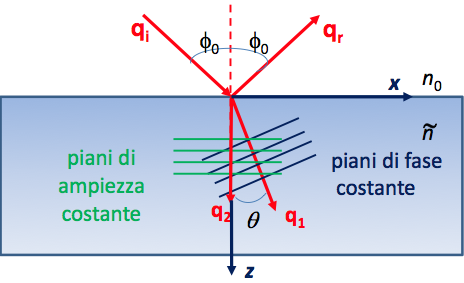
\includegraphics[width=3.5in]{immagini/rifaz.png}
\end{center}
Supponendo che, come in figura, $\widetilde \q$ giaccia nel piano $\(x,z\)$ e che il mezzo da cui l'onda incide sia il vuoto quindi $\sin{\phi_0}=\widetilde n\sin{\widetilde \phi}$. Le componenti complesse di $\widetilde \u$ sono:
\begin{equation}\begin{split}
\begin{cases}
\widetilde u_x=\sin{\widetilde \phi}=\sin{\frac{\phi_0}{\widetilde n}}\\
\widetilde u_y=0\\
\widetilde u_z=\cos{\widetilde \phi}=\sqrt{1-\sin^2{\widetilde \phi}}
\end{cases}
\end{split}\end{equation}

La \b{fase dell'onda}, dipendente da $\r$, è:
\begin{equation}\begin{split}
i\widetilde \q\cdot\r=\\
i\frac{\omega}{c}\(x\widetilde u_x+z\widetilde u_z\)=\\
i\frac{\omega}{c}\(x\sin{\frac{\phi_0}{\widetilde n}}+y\cos{\widetilde \phi}\)=\\
i\frac{\omega}{c}\(x\sin{\phi_0}+z\widetilde n\cos{\widetilde \phi}\)=\\
i\frac{\omega}{c}\[x\sin{\phi_0}+z\Re\(\widetilde n\cos{\widetilde \phi}\)+iz\Im\(\widetilde n\cos{\widetilde \phi}\)\]=\\
i\frac{\omega}{c}\[x\sin{\phi_0}+z\Re\(\widetilde n\cos{\widetilde \phi}\)\]-z\frac{\omega}{c}\Im\(\widetilde n\cos{\widetilde \phi}\)
\end{split}\end{equation}
dove l'ultimo termine a destra rappresenta lo smorzamento, che dipende solo da $z$: \b{le superfici di ampiezza costante sono piani perpendicolari a $z$}. Il termine $x\sin{\phi_0}+z\Re\(\widetilde n\cos{\widetilde \phi}\)+iz\Im\(\widetilde n\cos{\widetilde \phi}\)$ rappresenta la fase: i piani di fase costanti hanno la normale (cioè $\q_1$) che forma con la normale all'interfaccia un angolo $\theta$ tale che:
\begin{equation}\begin{split}
\tan{\theta}=\frac{\sin{\phi_0}}{\Re\(\widetilde n\cos{\widetilde \phi}\)}.
\end{split}\end{equation}

\subsubsection{Onda incidente polarizzata rettilineamente}
Il tipo di polarizzazione è lo stesso, anche se nella riflessione e nella rifrazione si ha una diversa rotazione del piano di polarizzazione.

\subsubsection{Onda incidente polarizzata ellitticamente}
Le onde riflessa e rifratta sono anch'esse polarizzata ellitticamente, ma l'eccentricità delle relative ellissi è diversa da quella dell'onda incidente perché i semiassi cambiano in modo diverso e il rapporto non si conserva.

\subsubsection{Onda incidente polarizzata circolarmente}
L'onda riflessa e l'onda rifratta non sono in genere circolari.

\subsection{Angolo di Brewster}
Si definisce l'\b{angolo di Brewster} come:
\begin{equation}\begin{split}
\tan{\theta_B}=\frac{n_2}{n_1}\\
\Longrightarrow \theta_B=\arctan{\frac{n_2}{n_1}}.
\end{split}\end{equation}

L'angolo di Brewster ha delle \b{proprietà caratteristiche}:
\begin{itemize}
\item esiste per qualsiasi coppia di valori di indici di rifrazione;
\item è sempre maggiore di \ang{45;;} se $n_1<n_2$ e sempre minore di \ang{45;;} se $n_1>n_2$;
\item dato che $\theta_B+\theta_{t,B}=\frac{\pi}{2}$, l'angolo tra il raggio riflesso e il raggio rifratto vale $\frac{\pi}{2}$;
\item determinati $\theta_B$ e il corrispondente angolo di rifrazione $\theta_{t,B}$, nel passaggio $n_1\to n_2$, $\theta_{t,B}$ e $\theta_B$ sono rispettivamente l'angolo di Brewster e l'angolo di rifrazione nel passaggio inverso $n_2\to n_1$.
\end{itemize}

\subsection{Polarizzazione per riflessione}
In condizioni di Brewster \b{la componente dell'onda incidente che vibra nel piano di incidenza viene totalmente trasmessa}, ma non viene riflessa e \b{la componente dell'onda che vibra nel piano ortogonale al piano di incidenza viene sia riflessa che trasmessa}.

Nella luce riflessa si trova solo la componente che vibra nel piano ortogonale: \b{per $\theta_i=\theta_B$ la luce riflessa è polarizzata rettilineamente nel piano ortogonale}. Il risultato è vero qualunque sia lo stato di polarizzazione dell'onda incidente.

\section{Propagazione di un'onda piana \elettrom in un mezzo anisotropo}%Propagazione di un'onda piana elettromagnetica in un mezzo anisotropo
Per dielettrici anisotropi (cristalli e materie plastiche artificiali, costituite da molecole lunghe e orientate preferibilmente in una certa direzione) \dP e \dD non sono generalmente paralleli ad $\E$.

La suscettività elettrica $\chi$ è considerata come un tensore simmetrico con sei componenti che valgono:
\begin{equation}\begin{split}
\begin{cases}
D_x=\e_0\[\(1+\chi_{11}\)E_x+\chi_{12}E_y+\chi_{13}E_z\]\\
D_y=\e_0\[\chi_{21}E_x+\(1+\chi_{22}\)E_y+\chi_{23}E_z\]\\
D_z=\e_0\[\chi_{31}E_x+\chi_{32}E_y+\(1+\chi_{33}\)E_z\]
\end{cases}
\end{split}\end{equation}
Lo stesso vale per la costante dielettrica relativa $\ke=1+\chi$.

\'E possibile, con una scelta opportuna degli assi $\(x,y, z\)$, diagonalizzare $\chi$ in modo che si abbiano solo le componenti $\chi_{ii}\neq0$, cioè si hanno in generale 3 valori per $\e_1$ ($\e_{xx}$, $\e_{yy}$, $\e_{zz}$) e 3 valori per $n$ ($n_1$, $n_2$, $n_3$):
\begin{equation}\begin{split}
\begin{cases}
D_x=\e_0\ke_1E_x\\
D_y=\e_0\ke_2E_y\\
D_z=\e_0\ke_3E_z
\end{cases}
\end{split}\end{equation}
Tali assi vengono detti \b{assi cristallografici}, o assi ottici o assi principali del dielettrico (dipendendo $\e_1$ da $\omega$, allora anche gli assi dipendono da $\omega$). Le costanti dielettriche si chiamano \b{costanti dielettriche relative principali}.

Nei mezzi anisotropi la densità di energia elettrica è $u_e=\frac{1}{2}\E\cdot\D$ e perciò si ha:
\begin{equation}\begin{split}
u_e=\frac{\frac{D_x^2}{\ke_1}+\frac{D_y^2}{\ke_2}+\frac{D_z^2}{\ke_3}}{2\e_0}.
\end{split}\end{equation}
\begin{center}
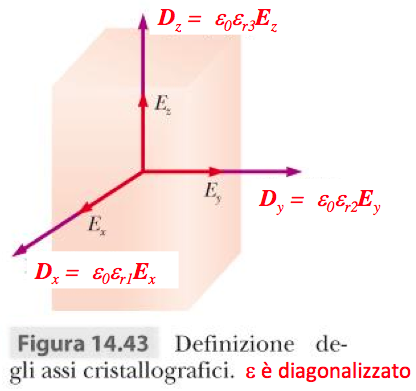
\includegraphics[width=3in]{immagini/assicrist.png}
\end{center}

Introducendo le variabili adimensionali $j=\frac{D_j}{\sqrt{2\e_0u_e}}$ si definisce l'\b{ellissoide degli indici di rifrazione del materiale}:
\begin{equation}\begin{split}
\frac{x^2}{n_1^2}+\frac{y^2}{n_2^2}+\frac{z^2}{n_3^2}=1
\end{split}\end{equation}
considerando che i tre semiassi sono $n_1=\sqrt{\ke_1}$, $n_2=\sqrt{\ke_2}$, $n_3=\sqrt{\ke_3}$.

Esistono tre categorie di cristalli esistenti in natura:
\begin{itemize}
\item Sostanze con $n_1=n_2=n_3=n$: l'ellissoide è una sfera di raggio pari a $n$ (materiale amorfo).
\item Sostanze con $n_1\neq n_2=n_3$: l'ellissoide è un ellissoide di rotazione intorno all'asse principale caratterizzato dall'indice di rifrazione $n_1$ (cristalli monoassici).
\item Sostanze con $n_1\neq n_2\neq n_3$: l'ellissoide non ha particolari simmetrie (cristalli biassici).
\end{itemize}
Mediante l'ellissoide degli indici è possibile trovare le velocità di fase e le direzioni di \dD corrispondenti a un dato $\k$.

\subsection{Cristalli monoassici}
Si usa indicare con il nome di \b{indice di rifrazione straordinario} ($n_s$) l'indice di rifrazione $n_1$ relativo all'asse ottico, mentre si indica col nome di \b{indice di rifrazione ordinario} ($n_o$) l'indice di rifrazione $n_2$ relativo ad un qualsiasi asse ortogonale all'asse ottico. Si ha quindi:
\begin{equation}\begin{split}
\frac{x^2}{n_s^2}+\frac{y^2+z^2}{n_o^2}=1.
\end{split}\end{equation}

Si distinguono in:
\begin{itemize}
\item \b{positivi} ($n_s>n_o$): l'ellissoide è allungato nella direzione dell'asse ottico;
\item \b{negativi} ($n_s<n_o$): l'ellissoide è schiacciato nella direzione dell'asse ottico.
\end{itemize}

\subsection{Impiego dell'ellissoide}
L'onda associata all'indice $n_o$ viene chiamata \b{onda ordinaria}: la polarizzazione è ortogonale all'asse ottico, i campi $\E_o$ e $\D_o$ sono sempre paralleli e stanno sul fronte d'onda, che è perpendicolare alla direzione di propagazione.

L'onda associata all'indice $n_s$ viene chiamata \b{onda straordinaria}: il campo elettrico $\E_s$ non è parallelo a $\D_s$ e non sta come questo sul fronte d'onda; $\E_s$ però è sempre ortogonale alla direzione di propagazione e pertanto fronte d'onda e direzione di propagazione non sono ortogonali tra loro.

Per qualsiasi orientazione del fronte d'onda rispetto all'asse ottico di un cristallo monoassico, si è in grado di determinare l'indice di rifrazione e la velocità di propagazione per un'onda polarizzata ortogonalmente all'asse ottico (onda ordinaria) e per l'onda a questa ortogonale, cioè polarizzata in un piano contenente l'asse ottico (onda straordinaria).

\subsection{Birifrangenza}
Supponendo un cristallo monoassico tagliato in modo da formare una lastra a facce piane e parallele e considerando un'onda luminosa piana non polarizzata che incide su una faccia del cristallo, si ha che in generale dal cristallo escono due onde separate, polarizzate rettilineamente lungo due direzioni tra loro perpendicolari, e l'insieme dei fatti osservati si spiega coerentemente ammettendo che all'interno del cristallo l'onda incidente si scinda nelle due onde suddette, le quali si propagano nel cristallo con velocità diverse e in direzioni diverse.

Un'onda è ordinaria e obbedisce alla legge di Snell: essa è polarizzata ortogonalmente all'asse ottico del cristallo. L'altra onda, quella straordinaria, non obbedisce alla legge di Snell ed è come se vedesse il cristallo con indice di rifrazione variabile con la direzione di propagazione tra due valori estremi $n_o$ e $n_s$.

Le \b{direzioni di propagazione} all'interno del cristallo dell'onda ordinaria seguono l'equazione:
\begin{equation}\begin{split}
x^2+y^2+z^2=v_o^2t^2.
\end{split}\end{equation}
Per l'onda straordinaria invece seguono l'equazione:
\begin{equation}\begin{split}
\frac{x^2}{v_o^2}+\frac{y^2+z^2}{v_s^2}=t^2
\end{split}\end{equation}
che è l'\b{ellissoide di rotazione attorno all'asse ottico}.

\section{Applicazioni della birifrangenza}%Applicazioni della birifrangenza

\subsection{Prisma di Nicol}
\'E composto da due lastre uguali di calcite tagliate e incollate tra loro con una resina chiamata balsamo del Canada, avente indice di rifrazione $n=1.55$ intermedio tra i due indici $n_o$ e $n_s$ della calcite. L'asse ottico sta nel piano di incidenza e non coincide con la normale alla faccia del cristallo con cui forma un angolo di \ang{45;;}.

Il raggio incidente non polarizzato si scinde in un raggio ordinario e in un raggio straordinario che si propagano in direzioni diverse (il raggio ordinario viene deviato di più di quello straordinario).

Il raggio ordinario, quando incontra la superficie di separazione tra calcite e balsamo di Canada, passa da un mezzo più rifrangente ad un mezzo meno, per i quali l'angolo limite di riflessione totale è di \ang{69;;}. Il raggio straordinario passa invece da un mezzo meno rifrangente a uno più rifrangente e non subisce riflessione totale.

L'onda uscente è polarizzata rettilineamente nel piano di incidenza.

\subsection{Cristalli dicroici}
Si consideri una lamina di sostanza monoassica tagliata parallelamente all'asse ottico, cioè a forma di lastra a facce piane e parallele tra loro e all'asse ottico, e un'onda piana luminosa non polarizzata che incide normalmente ad una faccia della lastra.

Nella lamina hanno origine un'onda ordinaria polarizzata ortogonalmente all'asse ottico e un'onda straordinaria polarizzata parallelamente. Entrambe si propagano nella direzione \dun dell'onda incidente.

Nella maggior parte dei cristalli monoassici si ha un'attenuazione trascurabile; esistono però in natura sostanze che assorbono in proporzioni molto diverse l'onda ordinaria e l'onda straordinaria: se le molecole che costituiscono la sostanza sono allungate si avrà un \b{grande assorbimento quando} il campo elettrico \b{\dE dell'onda è parallelo all'asse} della molecola e un \b{assorbimento molto minore quando \dE è perpendicolare all'asse}. Una delle due onde viene progressivamente assorbita e diffusa e se lo spessore è sufficiente praticamente scompare, mentre l'altra prosegue.

Tra le sostanze dicroiche ci sono la formalina (assorbe l'onda ordinaria) e l'erapatite. Cristalli di erapatite orientati parallelamente e impaccati tra due fogli di materiale trasparente, vetro e nitrocellulosa, costituiscono una lamina di materiale dicroico, detta \b{polaroid}. Esse assorbono in modo praticamente completo una componente e trasmettono oltre il 70\% dell'intensità dell'altra, nell'intervallo di lunghezze d'onda da \SI{0.5}{\um} a \SI{0.7}{\um}.

\b{Una lamina dicroica è un dispositivo che fornisce un'onda polarizzata rettilineamente lungo una direzione che si chiama asse ottico della lamina}.

\subsubsection{Legge di Malus}
L'onda incidente normalmente sul polarizzatore è polarizzata rettilineamente e il campo elettrico $\E_0$ forma un angolo $\theta$ con l'asse ottico del polarizzatore. Detta $I_0$ l'intensità dell'onda polarizzata incidente, proporzionale a $E_0^2$, l'intensità $I_1$ dell'onda uscente, polarizzata lungo l'asse ottico del polarizzatore, è proporzionale a $E_0^2\cos^2{\theta}$ e si può scrivere la \b{legge di Malus}:
\begin{equation}\begin{split}
I_1=I_0\cos^2{\theta}.
\end{split}\end{equation}
L'intensità uscente da un polarizzatore colpito da luce rettilineamente polarizzata varia proporzionalmente al quadrato del coseno dell'angolo tra la direzione di polarizzazione incidente e l'asse ottico del polarizzatore.

\subsubsection{Analizzatore}
Essendoci un'onda non polarizzata incidente normalmente su un polarizzatore e un'onda polarizzata uscente dal polarizzatore che incide a sua volta normalmente su un secondo polarizzatore detto analizzatore, si trova una proprietà caratteristica: ruotando l'asse dell'analizzatore così che l'angolo $\alpha$ tra gli assi ottici dei polarizzatori passi da 0 a $2\pi$, l'intensità trasmessa è massima per $\alpha=0$ e $\alpha=\pi$. \b{Con gli assi ottici paralleli si ha il massimo di trasmissione, con gli assi ottici incrociati la trasmissione è nulla}. Questo è valido solo se la luce è polarizzata rettilineamente; per luce ellittica si ha soltanto una variazione dell'intensità, che non si annulla mai, e negli altri due casi non si ha nessuna variazione.

\subsubsection{Intensità trasmessa dall'analizzatore}
\begin{tabularx}{13cm}{l| X X}
\toprule
\multirow{2}{*}{Polarizzazione} & 		Intensità & 				Intensità \\
 & 							incidente &				trasmessa \\
\midrule
Ellittica &						$I=I_y+I_z$ & 				$I_p\(\alpha\)=I_y\cos^2{\alpha}+I_z\sin^2{\alpha}$ \\[2ex]
Circolare &					$I_y=I_z=\frac{I}{2}$ & 		$I_p\(\alpha\)=\frac{I}{2}$ \\[2ex]
\multirow{2}{*}{Rettilinea} &			$I_y=I\cos^2{\theta}$ & 		\multirow{2}{*}{$I_p\(\alpha\)=I\cos^2{\(\theta-\alpha\)}$} \\[2ex]
 &							$I_z=I\sin^2{\theta}$ & 		\\[2ex]
Luce ordinaria &					$I_y=I_z=\frac{I}{2}$ & 		$I_p\(\alpha\)=\frac{I}{2}$ \\[2ex]
\bottomrule
\end{tabularx}

\subsection{Lamine di ritardo}
Lamina di cristallo monoassico non dicroico, caratterizzata dagli indici di rifrazione $n_o$ e $n_s$, tagliata con le superfici parallele all'asse ottico.

Se la lamina sta nel piano $\(y,z\)$ e l'asse ottico è parallelo all'asse $y$, se un'onda piana \elettrom polarizzata rettilineamente si propaga lungo l'asse $x$ e incide sulla lamina stessa, e indicando con $\theta$ l'angolo formato dal campo elettrico \dE con l'asse ottico, si può scrivere l'onda incidente come:
\begin{equation}\begin{split}
E_y=E_0\cos{\theta}\cos{\(kx-\omega t\)}\\
E_z=E_0\sin{\theta}\cos{\(kx-\omega t\)}
\end{split}\end{equation}
e, dopo aver attraversato la lamina di spessore $d$, l'onda diventa:
\begin{equation}\begin{split}
E_{\textrm{stra}}=E_y=E_0\cos{\theta}\cos{\(kx+k_sd-\omega t\)}\\
E_{\textrm{ord}}=E_z=E_0\sin{\theta}\cos{\(kx+k_od-\omega t\)}
\end{split}\end{equation}

Mentre le componenti dell'onda entrante sono in fase, la componente straordinaria e la componente ordinaria dell'onda uscente sono sfasate. Lo \b{sfasamento} è:
\begin{equation}\begin{split}
\Delta\phi=\phi_s-\phi_o=\(k_s-k_o\)d=k\(n_s-n_o\)d=\frac{2\pi}{\lambda}\(n_s-n_o\)d
\end{split}\end{equation}
e si vede che \b{l'onda straordinaria è in anticipo su quella ordinaria nei cristalli positivi, in ritardo in quelli negativi}. E si ha quindi l'onda uscente:
\begin{equation}\begin{split}
E_y=E_0\cos{\theta}\cos{\(kx+k_sd-\omega t\)}\\
E_z=E_0\sin{\theta}\cos{\(kx+k_sd-\omega t-\Delta\phi\)}
\end{split}\end{equation}

\subsubsection{Lamina quarto d'onda}
Lo sfasamento introdotto dalla lamina è un multipolo intero dispari di $\frac{\pi}{2}$:
\begin{equation}\begin{split}
\Delta\phi=\(2m+1\)\frac{\pi}{2}\\
d=\frac{\lambda}{4\(n_s-n_o\)}\(2m+1\), \qquad m=0,1,2,\dots
\end{split}\end{equation}
e trasforma un'onda polarizzata rettilineamente in un'onda polarizzata ellitticamente con gli assi dell'ellisse paralleli agli assi coordinati $y$ e $z$.

Se $\theta=\frac{\pi}{4}$ l'onda è polarizzata circolarmente con il campo elettrico costantemente uguale a $\frac{E_0}{\sqrt{2}}$.

Se l'onda incidente è polarizzata circolarmente esce dalla lamina polarizzata rettilineamente a \ang{45;;} rispetto all'asse ottico della lamina; se la polarizzazione è ellittica l'onda esce polaraizzata ad un angolo $\theta$ tale che $\tan{\theta}=\frac{E_{0,z}}{E_{0,y}}$.

\subsubsection{Lamina mezz'onda}
Lo sfasamento introdotto dalla lamina è un multipolo intero dispari di $\pi$:
\begin{equation}\begin{split}
\Delta\phi=\(2m+1\)\pi\\
d=\frac{\lambda}{2\(n_s-n_o\)}\(2m+1\), \qquad m=0,1,2,\dots
\end{split}\end{equation}
e trasforma un'onda polarizzata rettilineamente in un'onda polarizzata ancora rettilineamente ma ad un angolo $-\theta$ con l'asse ottico della lamina. Se l'onda ha una polarizzazione ellittica o circolare si ha semplicemente un'inversione del senso di rotazione.

Se lo sfasamento introdotto dalla lamina fosse un multiplo pari di $\pi$, la lamina sarebbe ininfluente. L'assorbimento è molto piccolo. \b{L'effetto della lamina si ha solo sullo stato di polarizzazione di un'onda piana polarizzata}.

\b{Se la luce incidente non è polarizzata, la lamina non ha nessun effetto}.

\section{Birifrangenza elettrica, magnetica e meccanica}%Birifrangenza elettrica, magnetica e meccanica
Quasi tutte le sostanze trasparenti isotrope diventano birifrangenti quando sono sottoposte ad un campo elettrico.

\subsection{Effetto Kerr}
La differenza tra gli indici di rifrazione straordinario e ordinario è:
\begin{equation}\begin{split}
n_s-n_o=K\lambda E^2
\end{split}\end{equation}
dove $K$ viene chiamata \b{costante di Kerr} e dipende inversamente dalla temperatura.

\subsubsection{Cella di Kerr}
Un condensatore piano ha come dielettrico nitrobenzolo e il sistema è posto tra due polarizzatori incrociati: in assenza di campo elettrico tra le armatura l'intensità trasmessa dal secondo polarizzatore è nulla. Quando si genera campo elettrico tra le armature, viene introdotto uno sfasamento $\Delta\phi=\phi_s-\phi_o=\(k_s-k_o\)d=k\(n_s-n_o\)d=\frac{2\pi}{\lambda}\(n_s-n_o\)d$ che diventa:
\begin{equation}\begin{split}
\Delta\phi=2\pi dKE^2.
\end{split}\end{equation}
\b{All'uscita della cella l'onda luminosa è polarizzata ellitticamente e il secondo polarizzatore trasmette solamente la componente parallela al suo asse ottico}.

Spegnendo il campo la trasmissione è bloccata e si può realizzare un \b{interruttore rapido} per un fascio luminoso.

\subsection{Effetto Pockels}
Alcune sostanze presentano un effetto analogo che però dipende linearmente dal campo elettrico e si verifica sia con una disposizione uguale a quella della cella di Kerr sia con il campo elettrico parallelo alla direzione di propagazione. Questo effetto \b{è usato per modulare o interrompere fasci luminosi} e trova applicazioni nel campo dei laser.

\subsection{Effetto Cotton-Mouton}
In vari liquidi si ha una birifrangenza magnetica che è massima quando \dB è ortogonale alla direzione di propagazione e segue la legge:
\begin{equation}\begin{split}
n_s-n_o=C\lambda B^2.
\end{split}\end{equation}

\subsection{Sollecitazioni meccaniche}
Materiali isotropi come il vetro e il plexiglas diventano birifrangenti se sottoposti a sollecitazioni meccanica. Si comportano come cristalli monoassici con asse ottico parallelo alla forza: la differenza $n_s-n_o$ è proporzionale alla pressione.

\section{Attività ottica}%Attività ottica
Alcune sostanze (dette destrogire o levogire) hanno la proprietà di ruotare la direzione di polarizzazione di un'onda luminosa piana polarizzata rettilineamente che lo attraversi. \'E posseduta da soluzioni di sostanze come lo zucchero, la canfora, la trementina e da cristalli come il quarzo. Essa è ricondotta a particolari forme di simmetria delle molecole, ma non alla loro disposizione all'interno della sostanza.

L'angolo di rotazione $\alpha$ della direzione di polarizzazione segue la legge:
\begin{equation}\begin{split}
\alpha=Kh
\end{split}\end{equation}
denominando $K$ come \b{potere rotatorio}.

\subsection{Legge di Biot}
Nelle soluzioni vale:
\begin{equation}\begin{split}
\alpha=kch=Kh
\end{split}\end{equation}
dove $c$ è la \b{concentrazione} e $k$ è il \b{potere rotatorio specifico della soluzione}.

\subsection{Effetto Faraday}
Alcune sostanze che non presentano attività ottica diventano otticamente attive quando sono sottoposte ad un campo magnetico. Vale la \b{legge di Verdet}:
\begin{equation}\begin{split}
\alpha=VBh\cos{\theta_B}
\end{split}\end{equation}
con $\theta_B$ l'angolo tra \dB e la direzione di propagazione dell'onda piana incidente polarizzata rettilineamente e $V$ è la \b{costante di Verdet}.

Tra l'attività ottica naturale e magnetica c'è una differenza importante: nel primo caso se la direzione di polarizzazione ruota di $\theta$ per un certo verso di percorrenza, la rotazione è di $-\theta$ per propagazione in verso opposto e un'onda che ripercorre il campione in due versi non subisce nessuna rotazione; nell'attività magnetica invece la rotazione è sempre dello stesso segno e risulterebbe $2\theta$ per un'onda che ripercorre il campione in due versi.

\section{Riflessione su una superficie metallica}%Riflessione su una superficie metallica
Per le alte frequenze, quando per l'indice di rifrazione si trova l'espressione $n^2=1-\frac{\omega_p}{\omega^2}$ considerando $\omega_p=\sqrt{\frac{Ne^2}{\e_0m_e}}$ la \b{pulsazione di plasma}. Si ha quindi il valore immaginario:
\begin{equation}\begin{split}
n=i\sqrt{\frac{\omega_p^2}{\omega^2}-1}=in_i.
\end{split}\end{equation}

In questa situazione non può esserci propagazione nel metallo. In condizioni di incidenza normale si ha che l'\b{intensità riflessa è uguale a quella incidente e non c'è trasmissione}:
\begin{equation}\begin{split}
\frac{E_r}{E_i}=\frac{n_1-n_2}{n_1+n_2}=\frac{1-in_i}{1+in_i}=\frac{\sqrt{1+n_i^2}e^{-i\phi}}{\sqrt{1+n_i^2}e^{i\phi}}=e^{-2i\phi}.
\end{split}\end{equation}

\subsubsection{Specchi}
Gli specchi sono costruiti con alluminio (o cromo) evaporato su vetro perché:
\begin{itemize}
\item il vetro protegge l'\ce{Al} dagli agenti ossidanti;
\item si può evaporare \ce{Al} per pochi \SI{}{\um};
\item evaporando l'\ce{Al} sul vetro, amorfo, ciò lo rende totalmente liscio e riflettente;
\item sia l'\ce{Al} che il \ce{Cr} sono molto riflettenti e abbastanza economici.
\end{itemize}

Il \ce{Cu} ha il suo colore perché riflette sotto i \SI{2}{\electronvolt} e perciò riflette bene il visibile dell'arancio-rosso.